\documentclass[11pt]{article}

\usepackage[margin=1in]{geometry}
\usepackage[T1]{fontenc}
\usepackage{lmodern}
\usepackage{amsmath,amssymb}
\usepackage{graphicx}
\usepackage{xcolor}
\usepackage{hyperref}
\usepackage{booktabs}
\usepackage{longtable}
\usepackage{listings}
\usepackage{caption}
\usepackage{float}

\hypersetup{
    colorlinks=true,
    linkcolor=blue,
    citecolor=blue,
    urlcolor=blue
}

\lstset{
    basicstyle=\ttfamily\small,
    breaklines=true,
    frame=single,
    columns=fullflexible,
    keepspaces=true
}

\title{Calibration of CDet Timing Offsets and ECal Time Dependence}
\author{Edward J. Brash\\
Christopher Newport University\\
Jefferson Lab SBS Collaboration}
\date{\today}

\begin{document}

\maketitle

\begin{abstract}
This note documents the procedure used to calibrate the timing response of the Coordinate Detector (CDet). The calibration proceeds in two main stages. First, channel-to-channel timing offsets are determined for each bar and applied to align the detector timing response across all channels. Second, a residual event-level timing dependence on the ECal ADC time is characterized with a linear fit and removed. A final global timing shift is then applied so that the corrected leading-edge timing distribution has a mean value of 30.0 ns. The purpose of this document is to provide a practical guide for graduate students performing or reproducing this calibration.
\end{abstract}

\tableofcontents
\newpage

\section{Introduction}

The Coordinate Detector (CDet) timing response exhibits two important systematic effects that must be corrected before high-quality physics analysis can be performed:

\begin{enumerate}
    \item channel-to-channel timing offsets between bars (or PMTs), and
    \item an event-level dependence of the CDet timing on the ECal ADC time.
\end{enumerate}

If these effects are left uncorrected, the timing distributions broaden significantly, which degrades coincidence timing resolution and complicates subsequent event selection.

This document summarizes the calibration procedure implemented in the ROOT analysis macros developed for this purpose. For each stage of the procedure, both the main ROOT command and the relevant plotting function call are recorded explicitly so that the analysis can be reproduced and modified as needed.

\section{Detector Organization}

The CDet consists of 168 bars organized as follows:

\begin{itemize}
    \item 2 layers,
    \item 2 sides per layer,
    \item 3 modules per side,
    \item 14 bars per module.
\end{itemize}

Thus,
\[
N_{\text{bars}} = 2 \times 2 \times 3 \times 14 = 168.
\]

The detector can be grouped as:

\begin{itemize}
    \item Layer 1 Left: bars 1--42
    \item Layer 1 Right: bars 43--84
    \item Layer 2 Left: bars 85--126
    \item Layer 2 Right: bars 127--168
\end{itemize}

Each bar corresponds to 16 TDC channels, so the bar number is determined from the electronic channel ID by
\[
\text{bar} = \left\lfloor \frac{\texttt{GoodElID}}{16} \right\rfloor.
\]

\section{General Timing Definitions}

For a given hit, the raw CDet timing is converted to nanoseconds according to
\[
t = t_{\mathrm{TDC}} \cdot C_{\mathrm{TDC}} - t_{\mathrm{ref}},
\]
where \(C_{\mathrm{TDC}}\) is the TDC calibration constant and \(t_{\mathrm{ref}}\) is the event reference TDC.

The calibration described here is applied to both the leading-edge (LE) and trailing-edge (TE) times.

\section{Step 1: Initial Timing Inspection}

The first step is to inspect the uncorrected timing response and verify that the standard elastic-event selection is working as expected.

\subsection{Main ROOT Command}

Replace the command below with the exact command used in your analysis.

\begin{lstlisting}
.x PlotElastic.C(3575,-1,0,0,5)
\end{lstlisting}

\subsection{Plotting Function Command}

Replace the function call below with the exact plotting command used to inspect the initial timing distributions.

\begin{lstlisting}
plotAllTDC()
\end{lstlisting}

\subsection{Purpose}

At this stage, one verifies that:
\begin{itemize}
    \item the global LE and TE timing distributions are populated,
    \item the event selection is producing a clean sample of good hits, and
    \item the timing spectra are sensible before any corrections are applied.
\end{itemize}

\section{Step 2: Determination of Per-Bar Timing Offsets}

The first calibration step is to determine the relative timing offset for each bar.

\subsection{Method}

A global leading-edge timing histogram,
\[
h_{\mathrm{AllGoodLE}},
\]
is filled using all good CDet hits, independent of bar number. Its mean value,
\[
\mu_{\mathrm{all}},
\]
is used as a reference.

For each bar \(i\), a separate histogram
\[
h_{\mathrm{BarGoodLE}}^{(i)}
\]
is filled, and its mean value
\[
\mu_i
\]
is extracted.

The bar timing offset is then defined as
\[
\Delta t_i = \mu_{\mathrm{all}} - \mu_i.
\]

This offset is the quantity that must be \emph{added} to the LE and TE times for that bar in order to align the bar with the detector average.

If the histogram for a given bar contains fewer than 20 entries, the offset is set equal to zero:
\[
\Delta t_i = 0.
\]

\subsection{Main ROOT Command}

Replace the command below with the exact macro invocation used for this stage.

\begin{lstlisting}
.x PlotElastic_with_barhist_offsets.C(3575,-1,0,0,5)
\end{lstlisting}

\subsection{Plotting Function Command}

Replace the function call below with the plotting function used to generate the global and per-bar timing histograms.

\begin{lstlisting}
plotAllTDC()
\end{lstlisting}

\subsection{Products of this Step}

This step produces:
\begin{itemize}
    \item the global histogram \(h_{\mathrm{AllGoodLE}}\),
    \item one histogram \(h_{\mathrm{BarGoodLE}}^{(i)}\) for each bar,
    \item a graph of timing offset versus bar number.
\end{itemize}

\subsection{Relevant Figures}

\begin{figure}[H]
    \centering
    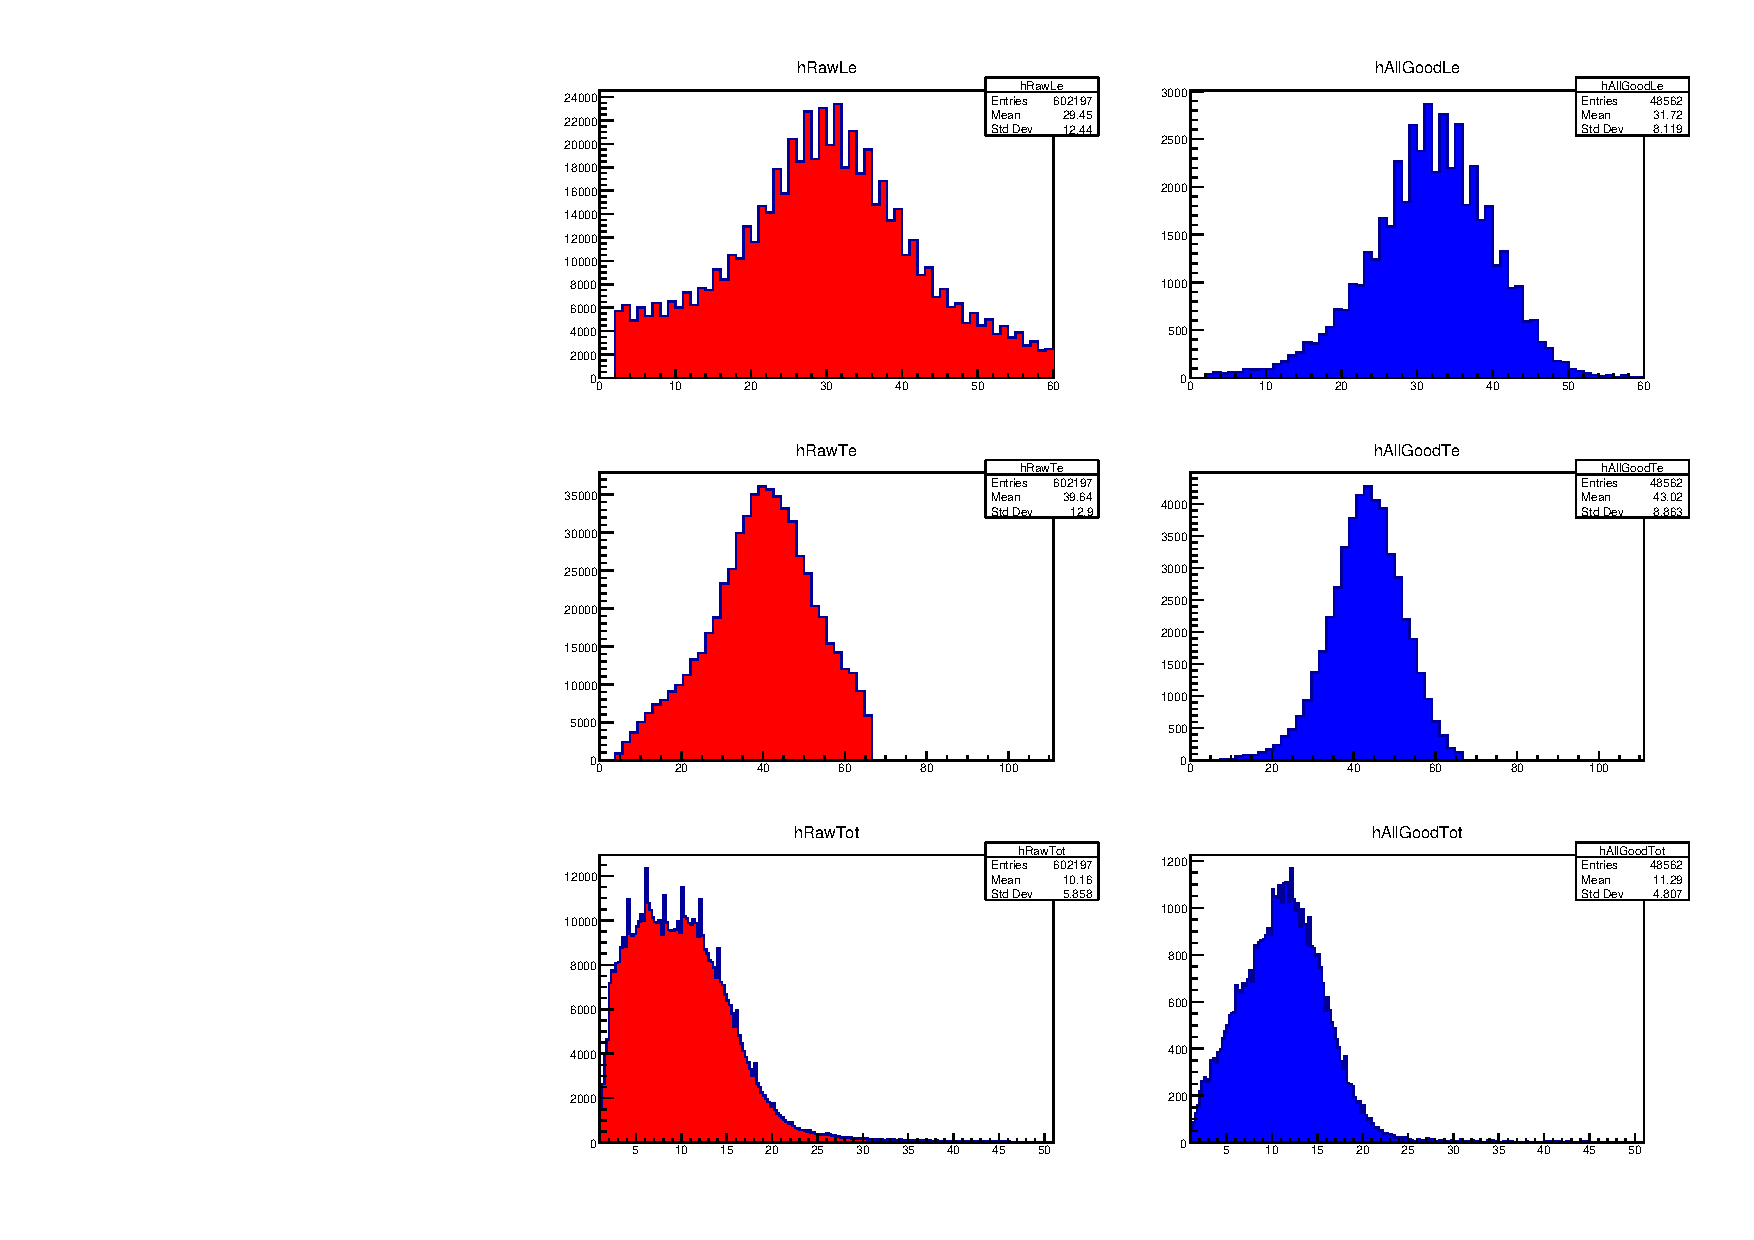
\includegraphics[width=0.8\textwidth]{figures/all_good_le.pdf}
    \caption{Global good leading-edge timing distribution used as the reference for the bar-by-bar offset calibration.}
\end{figure}

\begin{figure}[H]
    \centering
    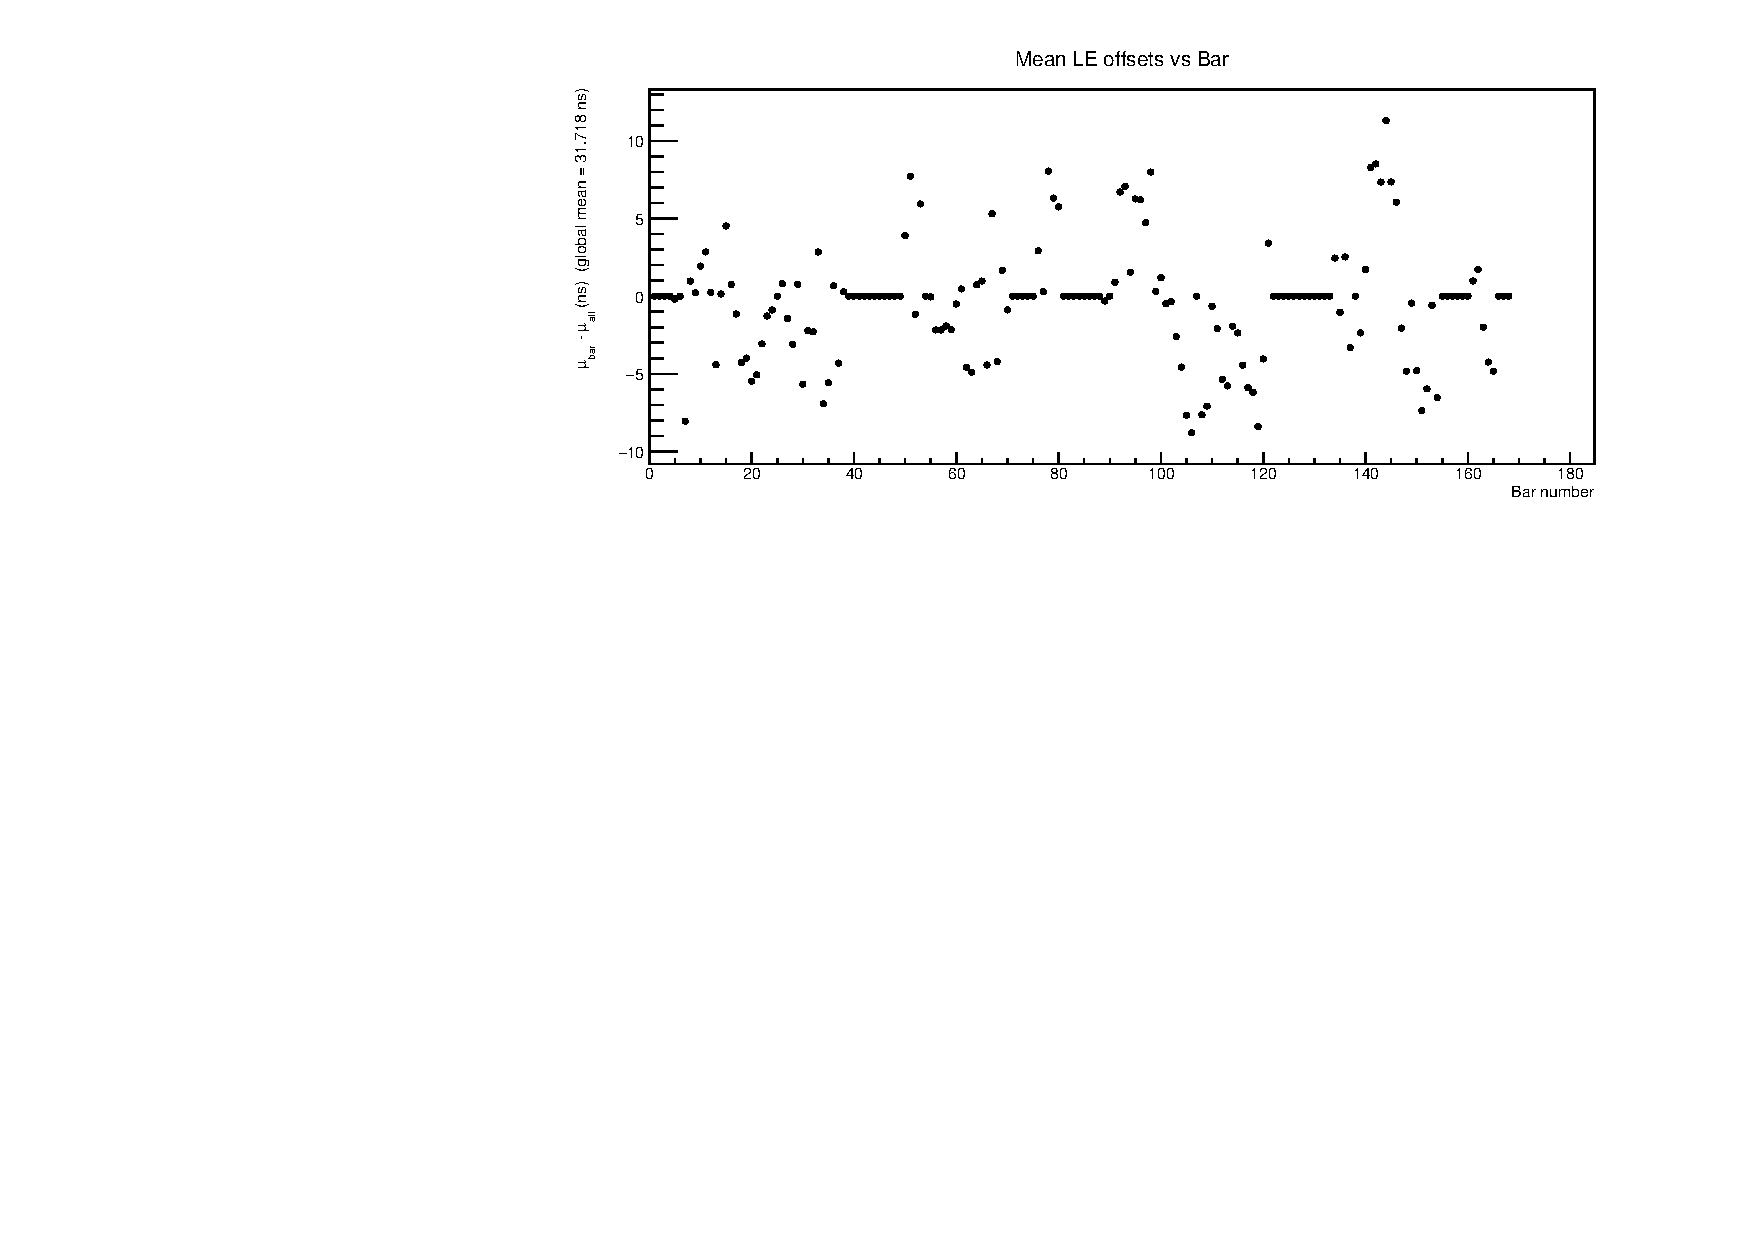
\includegraphics[width=0.9\textwidth]{figures/bar_offset_vs_bar.pdf}
    \caption{Timing offset as a function of bar number. Bars with fewer than 20 entries are assigned an offset of zero.}
\end{figure}

\section{Step 3: Visualization of Per-Bar Timing Histograms}

To inspect the timing spectra bar-by-bar in a physically meaningful layout, the 168 bars are displayed on four canvases.

\subsection{Canvas Organization}

The canvases are arranged as follows:

\begin{center}
\begin{tabular}{ll}
\toprule
Canvas & Bars \\
\midrule
Layer 1 Left & 1--42 \\
Layer 1 Right & 43--84 \\
Layer 2 Left & 85--126 \\
Layer 2 Right & 127--168 \\
\bottomrule
\end{tabular}
\end{center}

Each canvas is divided into a \(7 \times 6\) grid.

\subsection{Main ROOT Command}

Replace the command below with the exact command used for the macro version containing the canvas display logic.

\begin{lstlisting}
.x PlotElastic_with_barhist_display.C(3575,-1,0,0,5)
\end{lstlisting}

\subsection{Plotting Function Command}

\begin{lstlisting}
plotAllTDC()
\end{lstlisting}

\subsection{Purpose}

These canvases are useful for identifying:
\begin{itemize}
    \item missing or low-statistics channels,
    \item bars with large shifts relative to neighboring channels,
    \item non-Gaussian timing structure,
    \item possible hardware or threshold issues localized to individual modules.
\end{itemize}

\section{Step 4: Writing and Reading the Bar Offset File}

Once the per-bar offsets are determined, they are written to a plain-text file:
\begin{lstlisting}
CDet_bar_toffsets.dat
\end{lstlisting}

The format of the file is
\begin{lstlisting}
bar_number    offset_ns    entries
\end{lstlisting}

A typical line has the form
\begin{lstlisting}
25   -0.187   326
\end{lstlisting}

\subsection{Main ROOT Command}

Replace with the exact command used for the macro version that writes and reads the offset file.

\begin{lstlisting}
.x PlotElastic_with_barhist_offsets_io.C(3675,-1,0,0,5)
\end{lstlisting}

\subsection{Plotting Function Command}

\begin{lstlisting}
plotAllTDC()
\end{lstlisting}

\subsection{Application of the Correction}

If the file \texttt{CDet\_bar\_toffsets.dat} exists when the macro is run, the offsets are read in and applied to the LE and TE times according to bar number:
\[
t_{\mathrm{bar\text{-}corr}} = t_{\mathrm{raw}} + \Delta t_{\mathrm{bar}}.
\]

If the file does not exist, the macro sets all offsets to zero, proceeds normally, and generates the file at the end of the run.  The main point here is that at this point in the analysis, one should have a file called \texttt{CDet\_bar\_toffsets.dat}  that exists, and when the analysis is run a second time, one should see essentially zero time offsets in that relevant plot (i.e. Figure 2 above).

\section{Step 5: Study of the ECal Time Dependence}

After the bar offsets are applied, a residual dependence of the CDet timing on the ECal ADC time may remain.

To study this effect, a two-dimensional histogram is filled:
\[
h_{\mathrm{ECalVsCDetT}},
\]
with:
\begin{itemize}
    \item x-axis = event ECal ADC time,
    \item y-axis = corrected CDet timing.
\end{itemize}

In the present analysis, the event-level ECal time is
\[
t_{\mathrm{ECal}} = \texttt{v\_GoodECalAdcTime[ev]},
\]
where \texttt{ev} is the event number.

\subsection{Main ROOT Command}

Replace the command below with the exact macro invocation used at this stage.

\begin{lstlisting}
.x PlotElastic_with_barhist_offsets_io_ecalfit.C(3575,-1,0,0,5,20,40,5,40)
\end{lstlisting}

\subsection{Plotting Function Command}

Replace this with the exact plotting function used to display the ECal/CDet timing correlation.

\begin{lstlisting}
plotCDetLayersTimeComp(1,-15,15,-0.1,0.1,20,40,10,40,-15,15,0,60,0,80,62,130,-104,-60)
\end{lstlisting}

\subsection{Fit Procedure}

A linear fit is performed to the timing dependence:
\[
t_{\mathrm{CDet}} = p_0 + p_1 t_{\mathrm{ECal}}.
\]

In the present calibration, the fitted parameters were found to be
\[
p_0 = -70.555,
\qquad
p_1 = 0.91682.
\]

\subsection{Relevant Figures}

\begin{figure}[H]
    \centering
    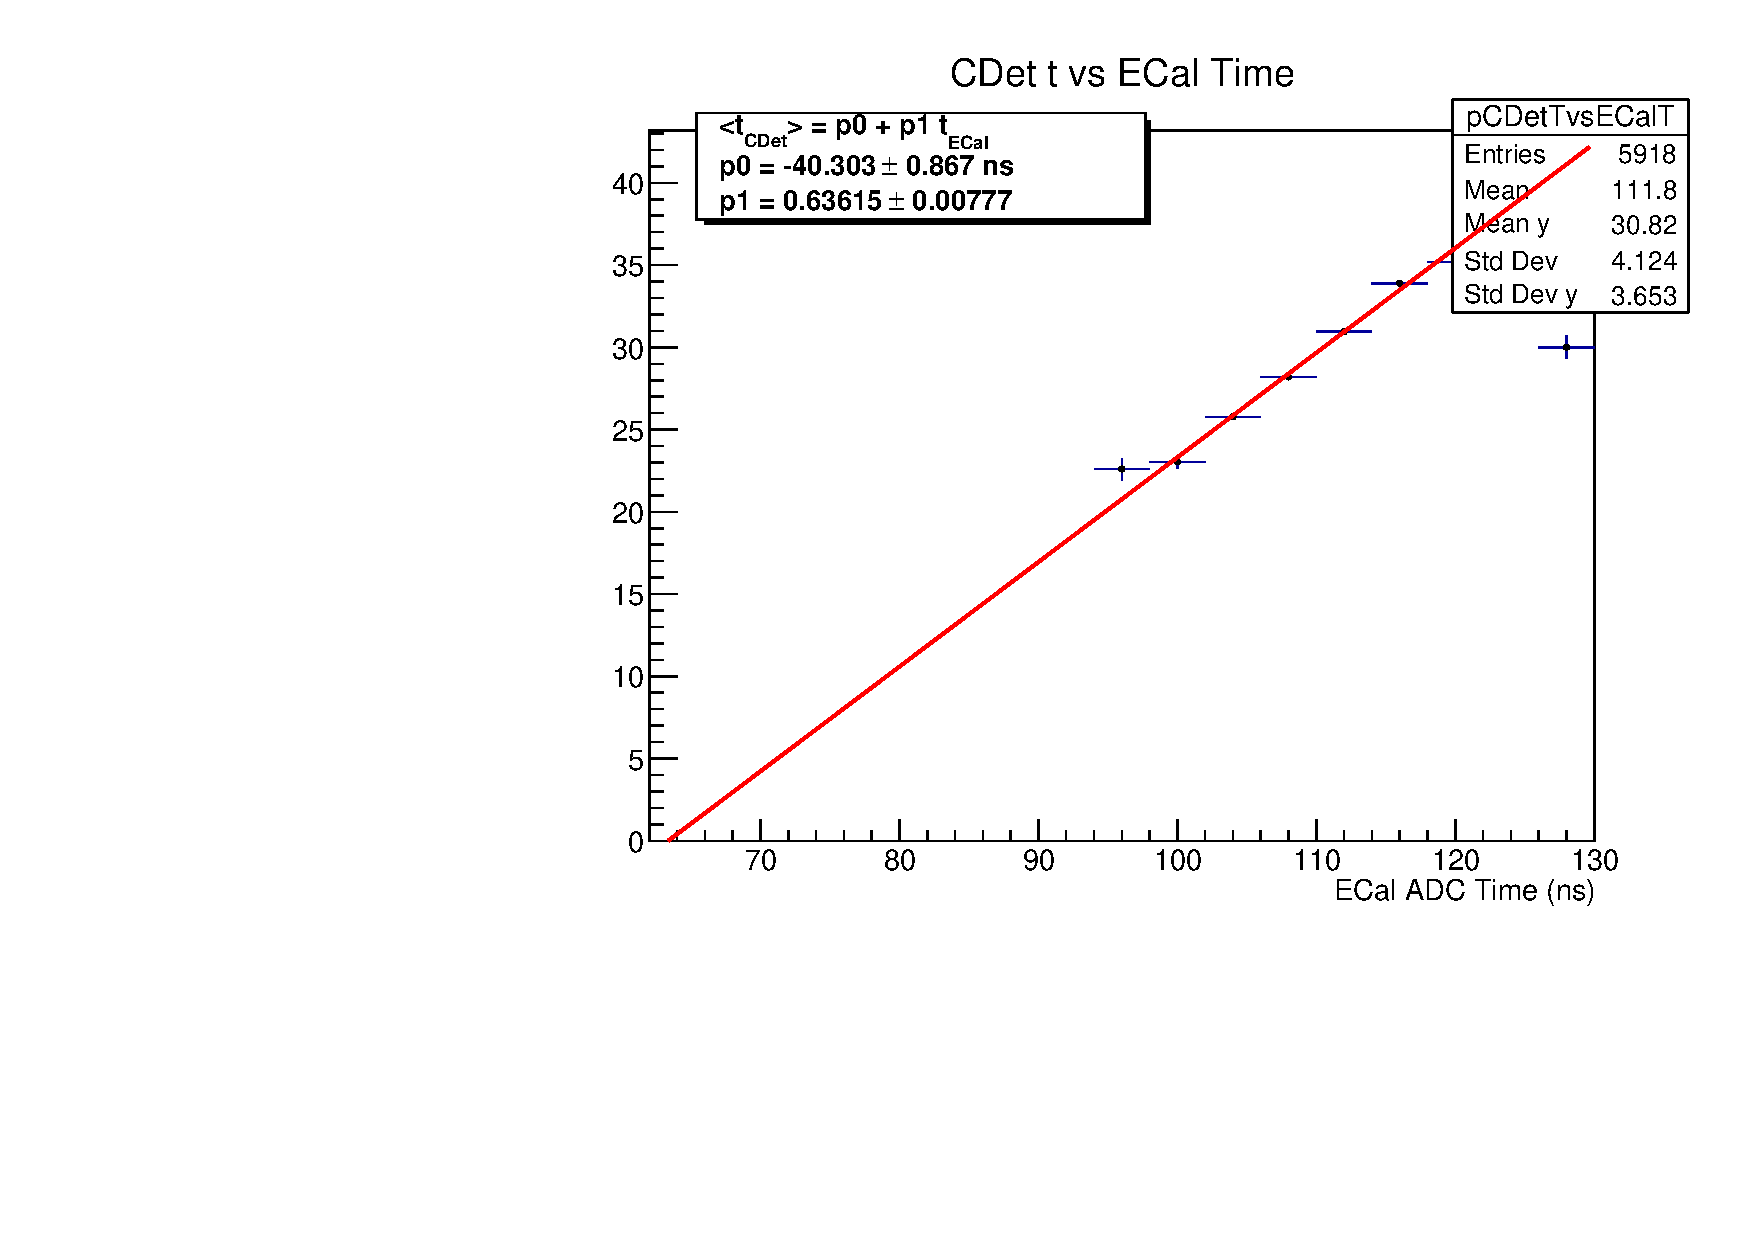
\includegraphics[width=0.75\textwidth]{figures/ecal_vs_cdet_fit.pdf}
    \caption{Two-dimensional plot of CDet time versus ECal ADC time, with profile and linear fit overlaid.}
\end{figure}

\section{Step 6: Application of the ECal Timing Correction}

After the linear dependence has been extracted, the next step is to remove it from the LE and TE times.

\subsection{Definition of the Correction}

Starting from the bar-corrected time,
\[
t_{\mathrm{bar\text{-}corr}} = t_{\mathrm{raw}} + \Delta t_{\mathrm{bar}},
\]
one defines the residual time
\[
t_{\mathrm{res}} = t_{\mathrm{bar\text{-}corr}} - (p_0 + p_1 t_{\mathrm{ECal}}).
\]

Using the fitted parameters obtained above,
\[
t_{\mathrm{res}} = t_{\mathrm{bar\text{-}corr}} - (-40.303 + 0.63615\, t_{\mathrm{ECal}}).
\]

\subsection{Global Shift to Set Mean LE Time to 30 ns}

After removing the ECal dependence, a final global shift is applied so that the mean corrected leading-edge time is 30.0 ns.

Let
\[
\mu_{\mathrm{res}} = \left\langle t_{\mathrm{res}} \right\rangle
\]
be the mean of the residual good leading-edge distribution. Then define
\[
\Delta = 30.0 - \mu_{\mathrm{res}}.
\]

The final corrected time is
\[
t_{\mathrm{corr}} = t_{\mathrm{res}} + \Delta.
\]

Thus the complete corrected time is
\[
t_{\mathrm{corr}}
=
t_{\mathrm{raw}}
+ \Delta t_{\mathrm{bar}}
- (p_0 + p_1 t_{\mathrm{ECal}})
+ \Delta.
\]

This correction is applied to both LE and TE times.

\subsection{Main ROOT Command}

Replace the command below with the exact macro invocation used to apply the full correction.

\begin{lstlisting}
.x PlotElastic_with_barhist_offsets_io_ecalcorr_apply.C(3575,3575,-1,0,0,5,20,40,5,40)
\end{lstlisting}

\subsection{Plotting Function Command}

Replace with the plotting function used to verify the fully corrected timing distributions.

\begin{lstlisting}
plotAllTDC()
plotCDetLayersTimeComp(1,-15,15,-0.1,0.1,20,40,10,40,-15,15,0,60,0,80,62,130,-104,-60)
\end{lstlisting}

\section{Step 7: Validation of the Final Calibration}

After the corrections are applied, the following checks should be performed:

\begin{enumerate}
    \item The global corrected LE histogram should have a mean near 30 ns.
    \item The per-bar histograms should be aligned with one another.
    \item The plot of CDet time versus ECal ADC time should show little or no residual slope.
    \item The coincidence timing resolution should be visibly improved relative to the uncorrected case.
\end{enumerate}

\subsection{Suggested Validation Figures}

\begin{figure}[H]
    \centering
    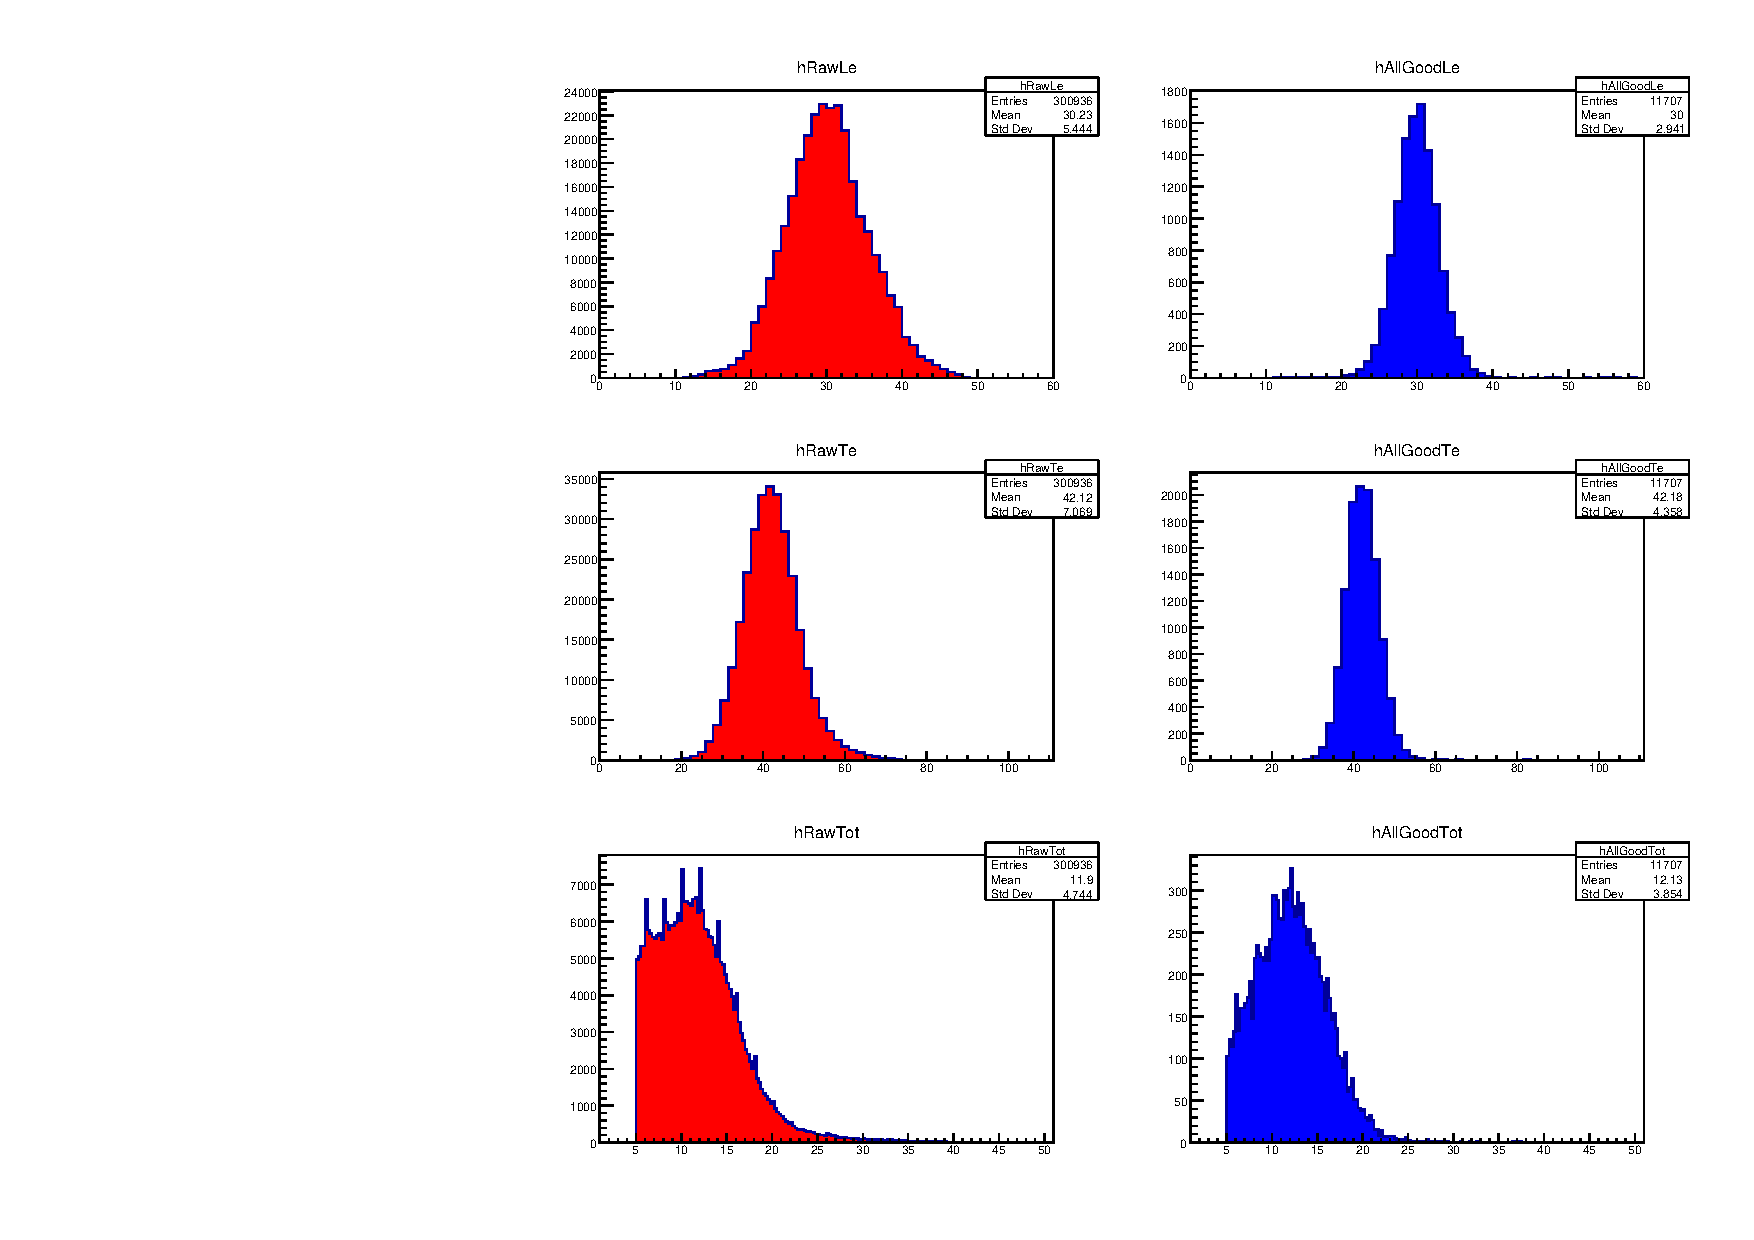
\includegraphics[width=0.8\textwidth]{figures/final_good_le.pdf}
    \caption{Final corrected good leading-edge timing distribution after application of both the per-bar and ECal time corrections.}
\end{figure}

\begin{figure}[H]
    \centering
    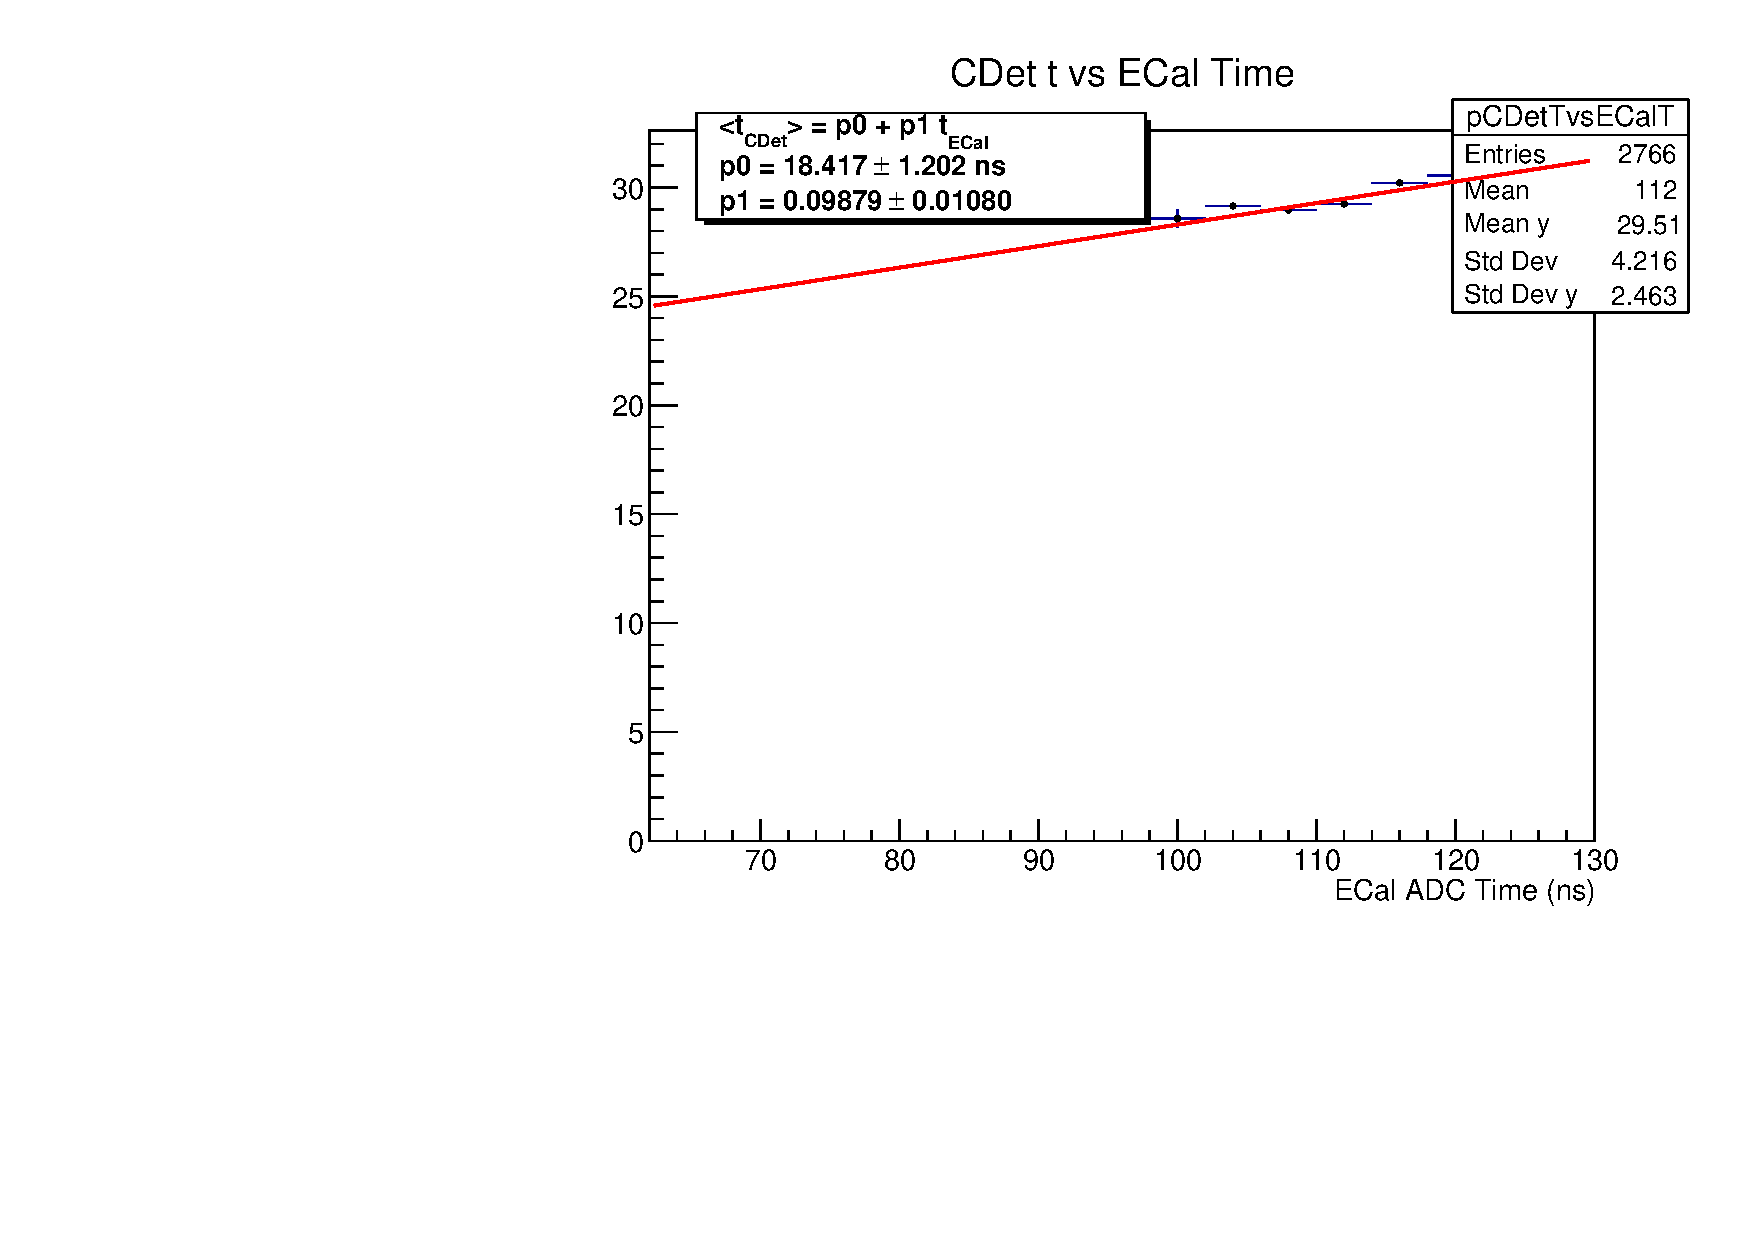
\includegraphics[width=0.75\textwidth]{figures/final_ecal_vs_cdet.pdf}
    \caption{Corrected CDet time versus ECal ADC time after removal of the fitted linear dependence.}
\end{figure}

\section{Practical Notes}

A few practical points are worth emphasizing:

\begin{itemize}
    \item Always verify that the event selection is stable before extracting timing offsets.
    \item Low-statistics channels should not be overinterpreted; the 20-entry threshold is intended to avoid unstable corrections.
    \item Be sure that the same definition of \(t_{\mathrm{ECal}}\) used in the fit is also used in the correction.
    \item The sign convention matters. In this analysis, the bar offset is defined as
    \[
    \Delta t_{\mathrm{bar}} = \mu_{\mathrm{all}} - \mu_{\mathrm{bar}},
    \]
    so the correction is applied by \emph{adding} this quantity to the raw timing.
    \item The ECal correction is applied after the bar correction.
    \item The final global shift is chosen only to place the corrected LE spectrum at a convenient mean value of 30.0 ns.
\end{itemize}

\section{Summary}

The CDet timing calibration described in this note consists of three conceptually distinct operations:

\begin{enumerate}
    \item determination and application of per-bar timing offsets,
    \item determination and removal of the event-level ECal timing dependence,
    \item application of a final global shift so that the corrected good LE distribution has mean 30.0 ns.
\end{enumerate}

The final corrected timing expression is
\[
t_{\mathrm{corr}}
=
t_{\mathrm{raw}}
+ \Delta t_{\mathrm{bar}}
- (p_0 + p_1 t_{\mathrm{ECal}})
+ \Delta.
\]

This procedure produces a substantially more uniform timing response across the detector and improves the overall timing quality for subsequent physics analysis.

\end{document}
